\chapter{Loop Accelerator Customization} \label{chapter:customization}
Despite the great advantages on design productivity, the additional layer on top of the physical FPGA inevitably imposes performance and resource consumption penalty. An overlay must ensure that the overall FPGA acceleration performance remains competitive. Otherwise, mapping the loop kernels to the overlay based FPGA accelerators will not be as useful. While a random SCGRA overlay configuration can rarely meet the performance requirements and the resource consumption budgets, therefore the capability to customize the overlay specifically to an application or a domain of application is essential to the overlay based FPGA accelerator design. However, navigating through a labyrinth of architectural and compilation parameters to fine-tune an accelerator's performance is a slow and non-trivial process. To require a user to manually explore such vast design space is going to counteract the productivity benefit of the utilizing overlay in the first place.

In order to address this problem, QuickDough can also automatically customize the overlay architectural parameters and exploit the optimized loop unrolling and hardware-software communication as well as buffer sizing specifically to a high-level compute intensive loop kernel with given high-level resource constraints. Most importantly, the customization makes all the hardware design and optimization details transparent to the users, which makes the whole system accessible to high-level designers. The user may choose to perform the customization only when the loop is changed dramatically and previous customization doesn't fit the updated loop kernel. In particular, by taking advantage of the regularity of the SCGRA overlay, a multitude of design metrics such as performance, hardware consumption and energy efficiency can be accurately estimated using analytical models once the overlay scheduling result is available. Since the overlay scheduling depends on much fewer design parameters, the overall customization framework can be dramatically simplified. With both the efficient application-specific customization and rapid compilation, the proposed design framework ensures both high design productivity and high performance of FPGA loop acceleration.

Application-specific customization provides unique opportunity to reduce the resource consumption and improve performance and energy efficiency of the resulting accelerators. However, taking the system as a black box and exhaustively searching all the possible configurations can be inefficient and slow. In this work, by taking advantage of the regularity of the SCGRA overlay based FPGA accelerator, we can reduce the complex customization problem to a much simpler sub design space exploration (DSE) together with a simplified search problem. With the customization, optimized application-specific nested loop accelerator can be produced efficiently.

\section{Customization Problem Formulation}
In this section, the customization problem of the nested loop acceleration on an SCGRA overlay based FPGA accelerator is formalized. Various design metrics including performance which is expressed as loop run time, energy consumption, energy efficiency and hardware resource consumption can either be used as the optimization goals or design constraints. However, the accelerator with smallest SCGRA overlay configuration and input/output data buffer apparently consumes the least FPGA resources while the resulting performance usually will not be acceptable, which is not quite useful in reality. Typically resource consumption will be used as design constraints instead of design goals. Energy consumption is not an appropriate design goal as well while the reason is not as obvious. As the power consumption model used in this work doesn't take the circuit activity into consideration, the power consumption is proportional to the SCGRA overlay size while the accelerator performance improves slower with the increase of the SCGRA overlay size. As a result, accelerator with a single PE will consume the least energy with little performance benefit. Basically both the energy consumption and the resource consumption are used as optional design constraints. In this formulation, performance is set to be the design goal while the rest metrics are used as design constraints. 

\begin{table}[htb]
    \centering
    \footnotesize
    \caption{Design Parameters of Nested Loop Acceleration
    \label{tab:parameter-list}}{
    \centering
    \begin{tabular}{l|l|l}
    \hline
    \multicolumn{2}{l|}{Design Parameters} & Denotation \\ \hline
    \multirow{2}{*}{\tabincell{l}{Nested Loop \\ Compilation}} & Loop Unrolling Factor &
    $\bm{u}=(u_0,u_1, ...)$  \\ \cline{2-3} 
                                                               & Grouping Factor & $\bm{g}=(g_0, g_1, ...)$ \\ \hline
    \multirow{12}{*}{\tabincell{c}{Overlay \\ Configuration}}  & SCGRA Topology  & 2D Torus, fixed \\ \cline{2-3} 
                                                               & SCGRA Size  & $r\times c$ \\ \cline{2-3}
                                                               & Data Width & $W_0$ \\ \cline{2-3}
                                                               & Data Mem & $D_0 \times W_0$ \\ \cline{2-3}
                                                               & Input Buffer & $D_1 \times W_0$ \\ \cline{2-3}
                                                               & Output Buffer & $D_2 \times W_0$ \\ \cline{2-3}
                                                               & Instruction Mem & $D_3 \times W_1$ \\ \cline{2-3}
                                                               & Input Address Buffer & $D_4 \times W_2$ \\ \cline{2-3}
                                                               & Output Address Buffer & $D_5 \times W_2$ \\ \cline{2-3}
                                                               & Operation Set & fixed \\ \cline{2-3}
                                                               & Implementation Frequency & $f$, fixed \\ \cline{2-3}
                                                               & Pipeline Depth & fixed \\ \hline
\end{tabular}
}
\end{table}

Suppose $\bm{\Psi}$ represents the overall nested loop acceleration design space. $\bm{C} \in \bm{\Psi}$ represents a possible configuration in the design space and it includes a number of design parameters as listed in \tabref{tab:parameter-list}. Assume that the loop to be accelerated has $n$ nested levels and loop count can be denoted as $l=(l_1, l_2, ..., l_n)$. $R=(R_1, R_2, R_3, R_4)$ stands for the FPGA resource (i.e. BRAM, DSP, LUT and FF) that are available on a target FPGA and $ResConsumption(\bm{C}, i)$ denotes the four different types of FPGA resource consumption. $Power(\bm{C})$ represents the power consumption. $Energy(\bm{C})$ and $EDP(\bm{C})$ are the estimated enegy consumption and energy delay product respectively while $Energy\_Budget$ and $EDP\_Budget$ are the corresponding budgets from the users. $In(\bm{g})$ and $Out(\bm{g})$ stand for the amount of input and output of a group. Similarly, $In(\bm{u})$ and $Out(\bm{u})$ stand for the amount of input and output of a DFG. $DFGCompuTime(\bm{C})$ represents the number of cycles needed to complete the DFG computation. $\alpha_i$ and $\beta_i$ are constant coefficients depending on target platform where $i=(1,2,...)$. With these denotations, the customization problem targeting minimum run time can be formulated as follows:

Minimize 
\begin{equation} \label{eq:runtime}
    RunTime(\bm{C})=CompuTime(\bm{C})+CommuTime(\bm{C})
\end{equation}
subject to
\begin{equation} \label{eq:constraints1}
    \begin{split}
        &ResConsumption(\bm{C}, i) \leq R_i, i=1,2,3,4 \\
        &Energy(\bm{C}) \leq Energy\_Budget \\
        &EDP(\bm{C}) \leq EDP\_Budget \\
    \end{split}
\end{equation}

\begin{equation} \label{eq:constraints2}
    \begin{split}
        &In(g) \leq D_1\\
        &Out(g) \leq D_2 \\
    \end{split}
\end{equation}

\begin{equation} \label{eq:constraints3}
    \begin{split}
        &\displaystyle \prod_{i=1}^{n} \frac{g_i}{u_i} \times In(u) \leq D_4 \\
        &\displaystyle \prod_{i=1}^{n} \frac{g_i}{u_i} \times Out(u) \leq D_5 \\
    \end{split}
\end{equation}

\begin{equation} \label{eq:constraints4}
DFGCompuTime(\bm{C}) \leq D_3
\end{equation}

The estimated hardware consumption, energy consumption and energy delay product should be within the budgets of the users, and the high-level constraints shown in \eqnref{eq:constraints1} should be fulfilled. On top of the basic high-level design constraints, there are a number of accelerator architectural constraints. As the accelerator transfers data in the granularity of a group, the input/output buffers should be able to accommodate all the input/output data of a group and constraints in \eqnref{eq:constraints2} should be satisfied. While the address buffers contain all the load/store addresses of DFGs in the same group, the total amount of the address buffers should be equal to or larger than the total amount of input/output of the DFGs in a group. As there may be data reuse between neghboring DFGs, the address buffer depth should be usually larger than the total amount of input/output of a group as shown in \eqnref{eq:constraints3}. The instruction memory stores the control words of every cycle of PEs. Therefore, the instruction memory depth should be equal to or larger than the number of cycles of DFG execution as shown in \eqnref{eq:constraints4}.

$RunTime(\bm{C})$ represents the number of cycles needed to compute the loop on the CPU-FPGA system. It consists of both the time consumed for computing on FPGA and communication between FPGA and host CPU. Assume there is no pre-fetching or overlap between computing and communication, and then $RunTime(\bm{C})$ can be calculated using \eqnref{eq:runtime}.

Since the unrolled part of the loop will be translated to DFG and then scheduled to the SCGRA overlay. Thus the DFG computation time is essentially a function of $\mathbf{u}$, $r$ and $c$, and it can also be denoted by $DFGCompuTime(\mathbf{u},r,c)$. The nested loop is computed by repeating the same DFG execution, and the nested loop computation can be calculated using \eqnref{eq:loopexetime}.

\begin{equation} \label{eq:loopexetime}
    CompuTime(\bm{C})=\displaystyle \prod_{i=1}^{n} \frac{l_i}{u_i} \times DFGCompuTime(\mathbf{u},r,c)
\end{equation}

DMA is typically used for the bulk data transmission. Communication cost per data can be modeled with a piecewise linear function and thus DMA latency can be calculated using $DMA(x)$ where $x$ represents the amount of DMA transmission. Assume the input data and output data are transferred sequentially, and then the communication time of the whole nested loop can be calculated by \eqnref{eq:commu}.
\begin{equation} \label{eq:commu}
    CommuTime(\bm{C})=\displaystyle \prod_{i=1}^{n} \frac{l_i}{g_i} \times 
    (DMA(In(\mathbf{g}))+DMA(Out(\mathbf{g})))
\end{equation}

On top of the performance model, we futher developed energy model and energy efficiency model. These models can be found in the appendix. 
 
\section{Customization Method}
To solve the customization problem as formalized in previous section, an automatic FPGA loop accelerator customization method based on the QuickDough compilation framework is presented as shown in \figref{fig:customization-framework}. 

The customization method can be roughly divided into two steps. In the first step, a sub DSE targeting loop execution time is performed and the feasible design space can be obtained. Since loop execution time is mostly determined by the operation scheduling which simply depends on the loop unrolling factor and SCGRA size, the sub DSE is much simpler compared to the overall system DSE which includes more than 10 design parameters. In the second step, each configuration in the feasible design space will be evaluated. Instead of using simulation based methods, analytical models as proposed in previous section are employed to estimate the accelerator metrics including performance, energy consumption, energy efficiency and hardware resource consumption. These analytical models are accurate because of the regularity of the SCGRA overlay. Even though the feasible design space is still large, it is very fast to evaluate all the configurations in it when compared to the time cost of the SCGRA scheduling process. After the evaluation process, customization for best performance becomes trivial and the optimized design parameters can be obtained immediately.

\begin{figure}[t]
\center{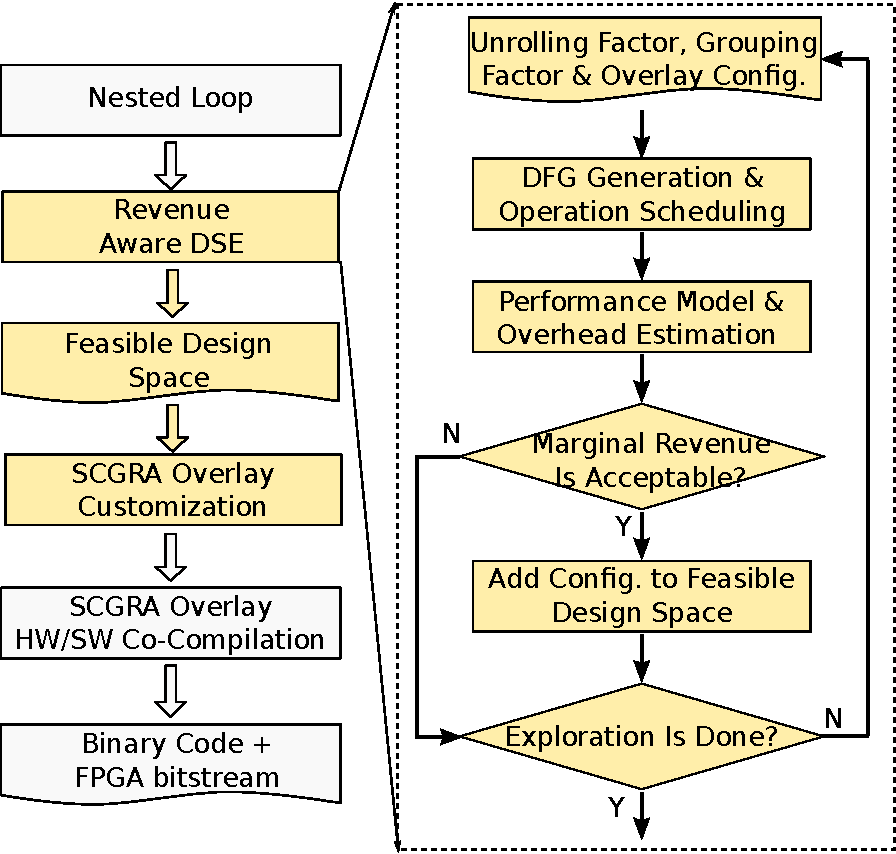
\includegraphics[width=0.6\linewidth]{customization-framework}}
\caption{Two-Step Customization Method}
\label{fig:customization-framework}
\end{figure}

\subsection{Sub Design Space Exploration}
The first step of the customization method is to perform the sub DSE for shorter loop computation time. As shown in \figref{fig:customization-framework}, this sub DSE focuses on the operation scheduler. The operation scheduling process is fast but not trivial. Although the sub DSE is already much simpler than the overall system DSE, it still requires to repeat the operation scheduling many times and straightforward sub DSE will take a large amount of time. Fortunately, it is clear that the operation scheduling only depends on the SCGRA overlay size and the loop unrolling factor. In addition, the two design parameters basically have monotonic influence on the DFG execution time according to our experiments as shown in \figref{fig:observation}. Typically both the larger loop unrolling factor and SCGRA size help to improve the performance of the DFGs mapped to the SCGRA overlay, though there are minor exceptions caused by the complex operation scheduling. Meanwhile, it can be found that the improvement slows down when the two design parameters get larger. When the improvement reaches a threshold, the increase of the design parameters has negligible influence on the DFG execution time. 

\begin{figure}[tb]
    \centering
    \subfigure[SCGRA Size]{%
      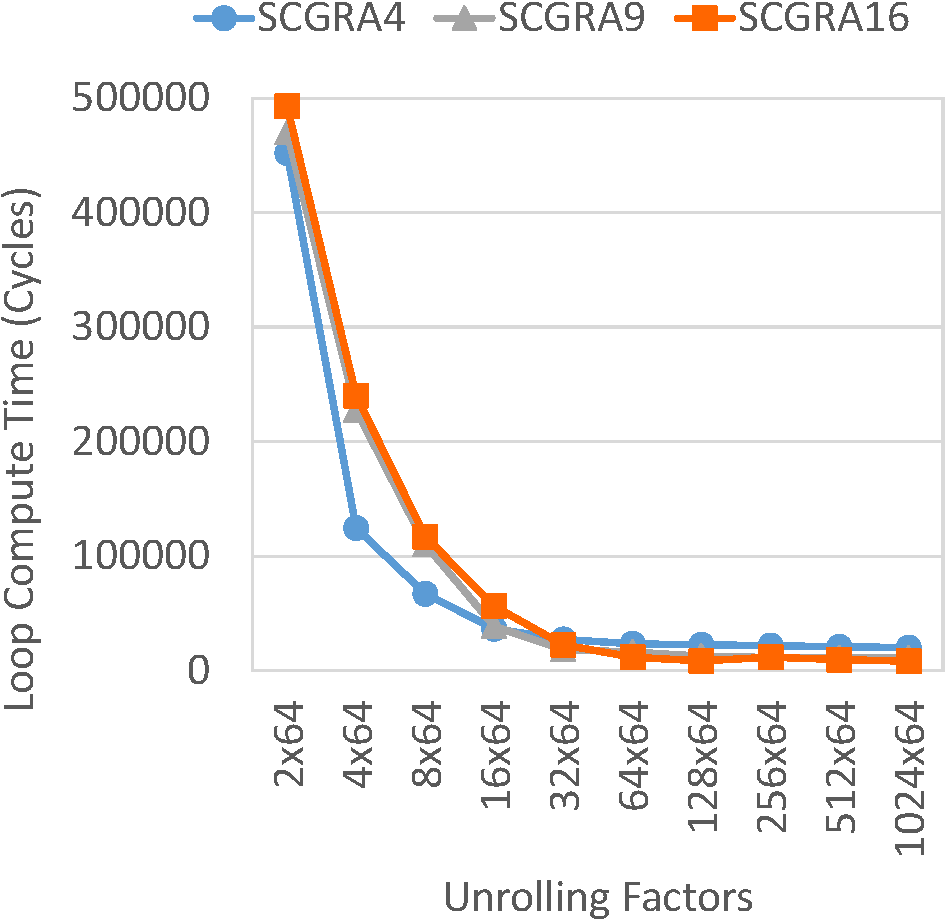
\includegraphics[width=0.42\textwidth]{scgrasize-perf}
      \label{fig:scgrasize-perf}
    }
    \hfill
    \subfigure[Loop Unrolling]{%
      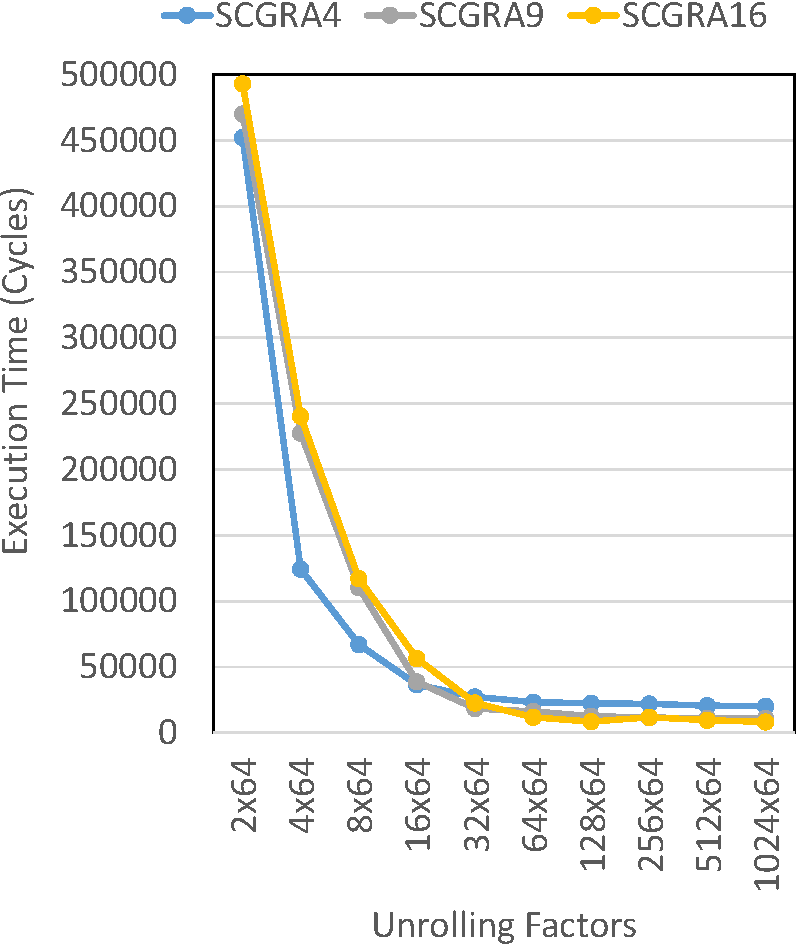
\includegraphics[width=0.42\textwidth]{unrolling-perf}
      \label{fig:unrolling-perf}
    }
    \caption{The design parameters typically have monotonic influence on the
        loop computation time and the computation time benefit degrades with 
    the increase of the design parameter. (a) SCGRA Size, the SCGRA topology used are torus with $2
\times 2$, $3 \times 2$, $3 \times 3$, ... while DFG-1, DFG-2 and DFG-3 are DFGs extracted from
matrix-matrix multiplication, fir and Kmean respectively. (b) Unrolling Factor, the loop used is a
63-tap Fir with 1024 input.} 
    \label{fig:observation}
  \end{figure}

With this observation, the feasible configurations must satisfy \eqnref{eq:cond1} and \eqnref{eq:cond2}, where $\Phi$ denotes the feasible design space and $\epsilon$ indicates the percentage of the performance benefit obtained by the increase of loop unrolling or SCGRA size. Whenever a configuration fails the sub DSE condition, all the configurations which are larger on one design parameter and remain the same on the rest design parameters can be safely pruned. Note that $\epsilon$ must be small enough to prune the configurations that are not worthwhile.

\begin{equation} \label{eq:cond1}
    \begin{split}
        &\forall \bm{C}=(...,\bm{u},r,c,...)\in \Phi, \bm{C'}=(...,\bm{u'},r',c',...) \in \Phi, \\
        & (r+1==r' \text{ and } c==c') \text{ or } (r==r' \text{ and } c+1==c'): \\ 
        &\frac{CompuTime(\bm{C})-CompuTime(\bm{C'})}{CompuTime(\bm{C})} > \epsilon \\
    \end{split}
\end{equation}

\begin{equation} \label{eq:cond2}
    \begin{split}
        &\forall \bm{C}=(...,\bm{u},r,c,...) \in \Phi, \bm{C'}=(...,\bm{u'},r,c,...) \in \Phi,\\ 
        &\bm{u} \text{ and } \bm{u'} \text{ are consecutive unrolling factors}: \\
        &\frac{CompuTime(\bm{C})-CompuTime(\bm{C'})}{CompuTime(\bm{C})} > \epsilon
    \end{split}
\end{equation}

In order to achieve the desired customization, the feasible design space defined by \eqnref{eq:cond1} and \eqnref{eq:cond2} must be able to cover the configuration that produces the optimal customization. A brief proof is presented as follows.

$\forall \bm{C'} \notin \Phi$, there must be a configuration $\bm{C}$ that fails \eqnref{eq:cond1} or \eqnref{eq:cond2}. Suppose $\bm{C'}=(...,\bm{u},r+1,c,...)$ and $\bm{C}=(...,\bm{u},r,c,)$. Thus it can be concluded that 

\begin{equation}
   CompuTime(\bm{C}) \geq  CompuTime(\bm{C'}) \geq (1-\epsilon) \times CompuTime(\bm{C})
\end{equation}

Since $\epsilon$ is small, $CompuTime(\bm{C'})$ is almost equal to $CompuTime(\bm{C})$. Meanwhile, the I/O buffer depth of both configurations are the same, so the $CommuTime(\bm{C'})$ is equal to $CommuTime(\bm{C})$. Therefore it can be concluded that $RunTime(\bm{C'}) \approx RunTime(\bm{C})$ according to \eqnref{eq:runtime}. In addition, as the unrolling factors of configuration $\bm{C}$ and $\bm{C'}$ are the same, $DFGCompuTime(\bm{C'}) \approx DFGCompuTime(\bm{C})$, which means that the instruction memory depth of configuration $\bm{C'}$ will be the same with that of configuration $\bm{C}$. While the increase of row size of the SCGRA overlay will result in significant BRAM consumption and power consumption. Thus $Power(\bm{C'}) \geq Power(\bm{C})$. As mentioned in previous paragraph, $RunTime(\bm{C'})$ is larger or equal to $RunTime(\bm{C})$. According to \eqnref{eq:energy}, it is clear that $Energy(\bm{C'}) \geq Energy(\bm{C})$. Taking all these design metrics into consideration, any configuration that is pruned during the sub DSE will not be an optimized configuration. Similarly, we can also draw the same conclusion when different occasions in \eqnref{eq:cond1} and \eqnref{eq:cond2} appear.

The sub design space exploration essentially aims to remove the configurations that will not be able to produce optimal design goals. As analyzed in previous paragraphs, instead of targeting the design goal directly, it simply focuses on the loop computing time which are mostly determined by the loop unrolling and SCGRA size. While the two design parameters have clear monotonic influence on the loop computing time, a simple branch and bound algorithm as detailed in \algref{alg:revenuealg} is used to explore the sub design space. It starts with a configuration with minimum SCGRA overlay size and unrolling factor. As a torus topology is used, the exploration analyzes the SCGRA row size, SCGRA column size and loop unrolling factor respectively. The increase of each parameter is evaluated using a revenue function $Revenue(\bm{C}, \bm{C'})$. When the revenue is larger than the pre-defined threshold, the configuration will be regarded as a feasible configuration and thus added to the feasible design space $\Phi$. 

\begin{algorithm}[hp]
\caption{Sub Design Space Exploration.}
\label{alg:revenuealg}
\begin{algorithmic}
\PROCEDURE{}
\STATE Initialize $r=2, c=2, \bm{u}=(1,1,...)$, feasible design space $\Phi=\emptyset$,
$\bm{C}=(...,r,c,\bm{u},...)$, maximum SCGRA overlay $r_{Max}\times c_{Max}$.
\WHILE {$r<r_{Max}$} 
\WHILE {$c<c_{Max}$}
\WHILE {$\bm{u}$ is not fully unrolled}
\STATE Generate DFG with $\bm{u}$
\STATE DFG Scheduling with configuration $\bm{C}$
\STATE Estimate performance $CompuTime(\bm{C})$
\STATE Get neighbor $\bm{C'} \in \Phi$ with smaller loop unrolling
\IF {$\bm{C'}$ exists and $Revenue(\bm{C}, \bm{C'}) \leq \epsilon$}
\STATE Break
\ELSE 
\STATE Add $\bm{C}$ to $\Phi$
\ENDIF
\STATE update $\bm{u}$ with larger neighbor unrolling factor
\ENDWHILE
\STATE Get neighbor $\bm{C''} \in \Phi$ with smaller column size
\IF {$\bm{C''}$ exists and $Revenue(\bm{C}, \bm{C''}) \leq \epsilon$}
\STATE Break
\ENDIF
\STATE $c=c+1$
\ENDWHILE
\STATE Get neighbor $\bm{C'''} \in \Phi$ with smaller row size
\IF {$\bm{C'''}$ exists and $Revenue(\bm{C}, \bm{C'''}) \leq \epsilon$}
\STATE Break
\ENDIF
\STATE $r=r+1$
\ENDWHILE
\ENDPROCEDURE
\STATE
\PROCEDURE {$Revenue(\bm{C}, \bm{C'})$}
\STATE return $\frac{CompuTime(\bm{C'})-CompuTime(\bm{C})}{CompuTime(\bm{C'})}$ 
\ENDPROCEDURE
\end{algorithmic}
\end{algorithm}

\subsection{Overall Customization}
The second step is to perform the overall FPGA loop accelerator customization and to produce the optimized FPGA loop accelerator. As the sub DSE in the first step have already determined a set of loop unrolling and SCGRA overlay size that may provide the optimized FPGA loop accelerator, this step focuses on the rest of the parameters of the FPGA loop accelerator including loop grouping, input/output buffer capacity, input/output address buffer capacity as well as instruction memory capacity. 

Given feasible loop unrolling and SCGRA overlay size, the number of cycles that is needed to complete the DFG extracted from the unrolled loop on the specified SCGRA overlay is immediately available. Then the optimized instruction memory depth which is larger or equal to the cycle count of the DFG execution can be obtained. Meanwhile, loop grouping which repeats the unrolled loop multiple times can be further explored. Given a possible loop grouping, the input/output data buffer capacity which is equal to or larger than the amount of input/output of the group can be thus decided. 

While the address buffer capacity is relatively difficult to decide, it is equal to or larger than the amount of the loop iteration input/output multiplied by the number of loop iterations (i.e. the unrolled loop body) included in each group. The depth of the address buffer is typically larger than that of the corresponding data buffer depending on the input/output data reuse between neighboring loop iterations. When there is no data reuse, the address buffer depth should be equal to that of the corresponding data buffer. When all the input data are reused and each loop iteration accesses the input data differently, then the input address buffer depth is $n$ times larger where $n$ is the number of loop iterations in the group. Note that the memories of the SCGRA overlay based FPGA accelerator are constructed using primitive block RAMs of the FPGA devices, so these memory capacity should be able to be divided by the primitive block RAM capacity. 

When all the potential configurations are decided, design goals including performance, energy consumption, energy efficiency can be estimated using the models proposed in previous section. Finally, the configuration that produce the optimal design goals is thus considered to be the customized configuration. In addition, when the customized configuration is decided, both the FPGA loop accelerator and the corresponding loop accelerator interfaces will be generated providing a complete hardware accelerator solution to the user. As the overall customization step searches through the feasible design space mostly based on the analytical models, the run time is negligible to that spent in the first step.

In addition, as all the design metrics of the feasible design metrics can be rapidly obtained, it is also possible to present a series of Pareto-optimal design spaces such as Energy-Performance and Resource Consumption-Performance allowing the users to make the final decision. 

\section{Experiments}
The experiments mainly include two parts. In the first part, the implementations of the SCGRA overlay based FPGA accelerators with different configurations are analyzed to demonstrate the regularity of the SCGRA overlay based FPGA accelerators, which are the basis of the proposed models. In the second part, both the efficiency and quality of the proposed customization framework is evaluated. In the experiments, the time consumption of the loop accelerator customization using the proposed two step customization is measured and compared to that of an exhaustive search. Then the performance speedup over a hard ARM processor is also presented. Meanwhile, the performance of the resulting accelerators generated using both the proposed customization and an exhaustive search are also compared. 

\subsection{Experiment Setup}
The customization run-time was obtained using a computer with Intel(R) Core(TM) i5-3230M CPU and 8GB RAM. Zedboard which has an ARM processor and an FPGA was used as the computation system. PlanAhead 14.7 was used for the SCGRA overlay based design. As the customization relies on analytical models instead of physical implementations, all the overlay implementations on Zedboard is assumed to work at 250MHz. To perform the customization, $\epsilon$ is set to be 0.05 and all the resource on Zedboard is set to be the resource budget. Software run-time is obtained from ARM processor of Zedboard.

In this section, four applications including Matrix Multiplication (MM), FIR, Kmean(KM) and Sobel Edge Detector (SE) are used as the benchmark. The configurations of the benchmark are the same with that detailed in the experiments in \chapref{chapter:framework}. 

\subsection{Customization Time}
Although customization is not a frequent process of QuickDough, it is also important to the productivity of the designers. \figref{fig:DSE-Time} shows the customization time of both the proposed two step (TS) customization and an exhaustive search based customization (ES). TS typically completes the customization in 10 minutes to 20 minutes and it is around 100X faster than the ES on average. In particular, ES is extremely slow on MM which has three levels of loop with relatively large loop count and thus larger design space. Though TS does need a dozen of minutes to complete the customization, it skips most of the unfeasible configurations and the run time is less sensitive to the size of the design space. 

\begin{figure}[htb]
    \centering
    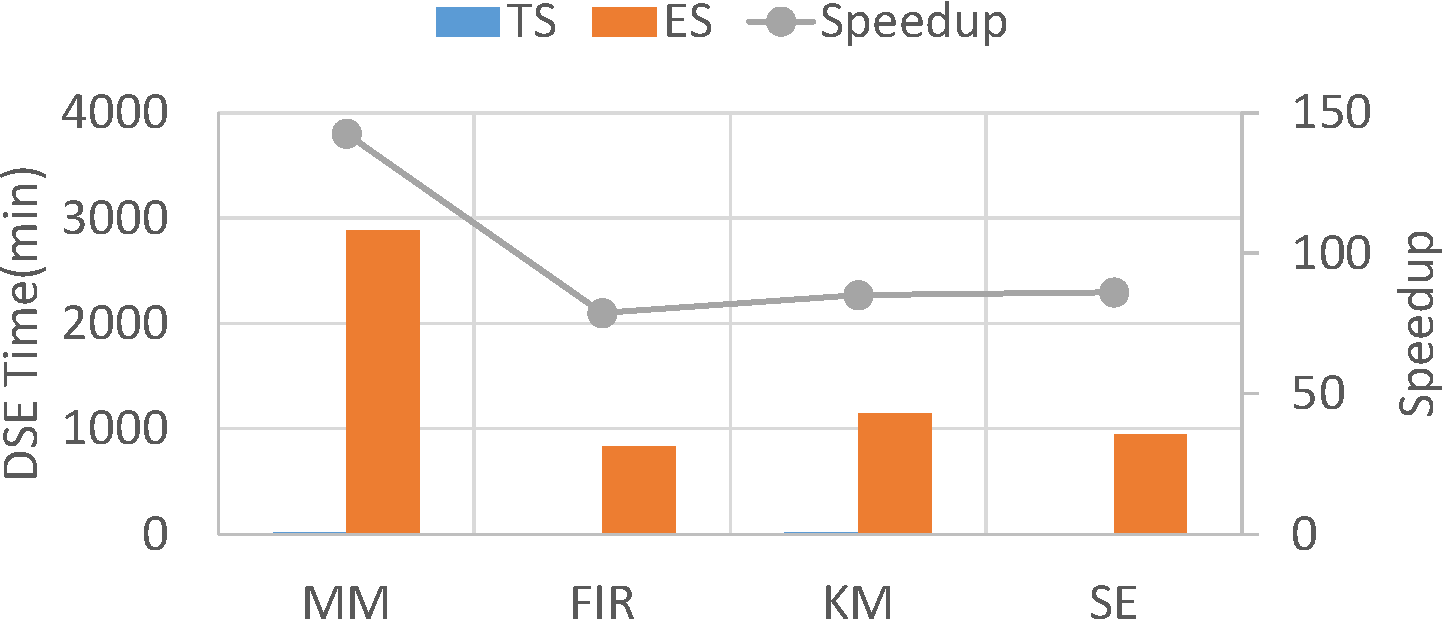
\includegraphics[width=0.65\textwidth]{DSE-Time}
    \caption{Customization Time Using Both TS and ES}
    \label{fig:DSE-Time}
\end{figure}

%\begin{table}[tb]
%    \small
%    \centering
%    \caption{Time Cost for RA DSE and ES DSE\label{tab:dsetime}}{
%        \begin{tabular}{l|l|l|l|l}
%            \hline
%            Benchmark & MM & FIR & KM & SE \\ \hline
%            RA DSE (min) & 20.2 & 10.6 & 13.4 & 11.4\\ \hline
%            ES DSE (min) & 2880.6 & 835.2 & 1140.5 & 946.2\\ \hline
%            Speedup & 142.6 & 78.8 & 85.1 & 86.2 \\ \hline
%        \end{tabular}
%    }
%\end{table}

In order to evaluate the sensitivity of the threshold $\epsilon$ to the customization, both of the customization time and the resulting accelerator run-time is analyzed with a set of different $\epsilon$ setup. \figref{fig:epsilon-sensitivity} shows the influence of the $\epsilon$ on the customization of FIR. When the $\epsilon$ is large, the customization time is much faster while the resulting accelerator performance is not optimized. On the other hand, smaller $\epsilon$ typically helps to produce accelerators with shorter runtime of accelerators, but customization time increases dramatically. In particular, when $\epsilon$ is small enough and optimized accelerator has already been found, even smaller $\epsilon$ will not lead to accelerators with better performance. Experiments on the rest of the applications show similar results and they are omitted to save the space. The optimal $\epsilon$ is up to the target application, while 0.05 works fine for all the applications in this benchmark.

\begin{figure}[htb]
    \centering
    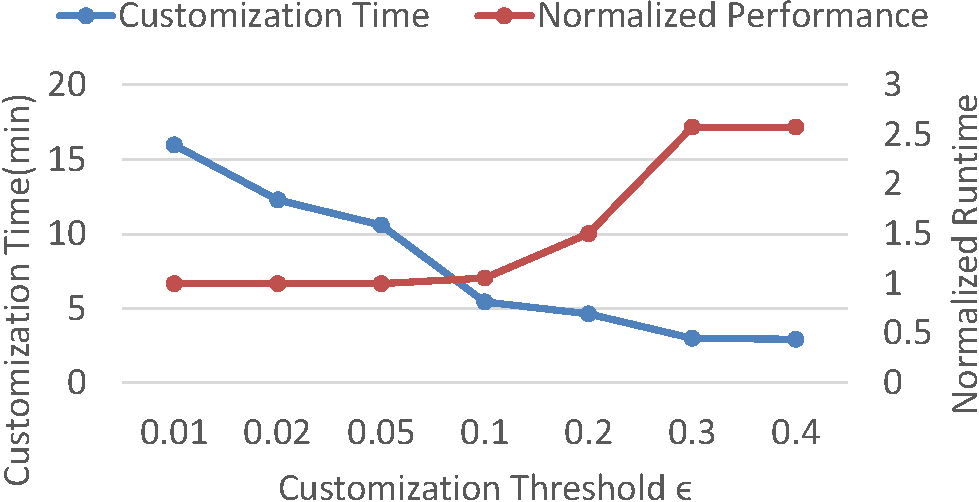
\includegraphics[width=0.65\textwidth]{epsilon-sensitivity}
    \caption{$\epsilon$ Influence on FIR Customization Time and Resulting Accelerator Run-time}
    \label{fig:epsilon-sensitivity}
\end{figure}
 
\subsection{Customized Accelerator Performance}
The proposed design framework will not be as useful if the performance of the generated system fails to provide competitive performance speedup over a general purpose processor which software designers can easily work with. Therefore, the computer kernel run-time on an ARM processor is presented as a basic comparison. In addition, in order to demonstrate both the necessity of the customization and the quality of proposed two-step customization method, the performance of the accelerators with a random configuration and customized configurations obtained using ES are compared with the performance of the accelerators customized using the proposed TS method. The detailed configurations of the accelerators are listed in \tabref{tab:acc-config}. Basically, the random configurations may come from an user who doesn't quite understand the underlying overlay architectures. The configurations generated using ES may cover all the possible configurations. The configurations generated using TS only explores the representative configurations expressed by the proposed models.

\begin{table}[htb]
    \footnotesize
    \centering
    \caption{Accelerator configurations (Note that the configurations include loop unrolling factor, grouping factor, SCGRA array size, instruction memory depth and IO buffer depth) \label{tab:acc-config}}{
        \begin{tabular}{l|l|l}
            \hline
            \multirow{3}{*}{MM}  & Base & ($1 \times 2 \times 100$, $4 \times 2 \times 100$, $5
        \times 5$, 1k, 2k)\\ \cline{2-3}
                                 & TS & ($1 \times 5 \times 100$, $50 \times 5 \times 100$, $4
        \times 4$, 1k, 8k)\\ \cline{2-3}
                                 & ES & ($1 \times 5 \times 100$, $25 \times 5 \times 100$, $5
        \times 4$, 1k, 8k)\\ \hline
            \multirow{3}{*}{FIR}  & Base & ($ 10 \times 50$, $100 \times 50$, $3
        \times 3$, 1k, 2k)\\ \cline{2-3}
                                 & TS & ($50 \times 50$, $2000 \times 50 $, $4
        \times 4$, 1k, 4k)\\ \cline{2-3}
                                 & ES & ($100 \times 50$, $5000 \times 50$, $5
        \times 4$, 1k, 8k)\\ \hline
            \multirow{3}{*}{SE}  & Base & ($4 \times 4 \times 3 \times 3$, $128 \times 128 \times 3
        \times 3$, $3 \times 2$, 1k, 8k)\\ \cline{2-3}
                                 & TS & ($16 \times 16 \times 3 \times 3$, $128 \times 128 \times 3
        \times 3$, $4 \times 4$, 1k, 4k)\\ \cline{2-3}
                                 & ES & ($16 \times 16 \times 3 \times 3$, $128 \times 128 \times 3
        \times 3$, $5 \times 4$, 1.5k, 4k)\\ \hline
            \multirow{3}{*}{KM}  & Base & ($25 \times 4 \times 2$, $2500 \times 4 \times 2$, $4
        \times 3$, 1k, 8k)\\ \cline{2-3}
                                 & TS & ($125 \times 4 \times 2$, $625 \times 4 \times 2$, $5
        \times 5$, 1k, 2k)\\ \cline{2-3}
                                 & ES & ($125 \times 4 \times 2$, $625 \times 4 \times 2$, $5
        \times 5$, 1k, 2k)\\ \hline

        \end{tabular}
    }
\end{table}

The performance comparison is shown in \figref{fig:DSE}. It is clear that random configuration is usually far from the optimized configuration. Therefore, customization is needed to provide meaningful FPGA loop accelerators. The customized accelerators obtained using TS achieves up to 10X speedup over the ARM processor on the benchmark. Particularly, the customized accelerator For FIR, SE and KM, the speedup is promising. MM has relatively low compute-IO rate and the single input and output between the on-chip buffer and the SCGRA overlay limits the performance of the accelerator. This problem can hopefully be alleviated by appropriate on-chip buffer partition, which will be supported in the proposed framework in future. Meanwhile, it can also be found that the performance of the accelerators customized using TS is quite close to the performance of that customized using ES. 

\begin{figure}[htb]
\centering
	\subfigure[MM]{%
		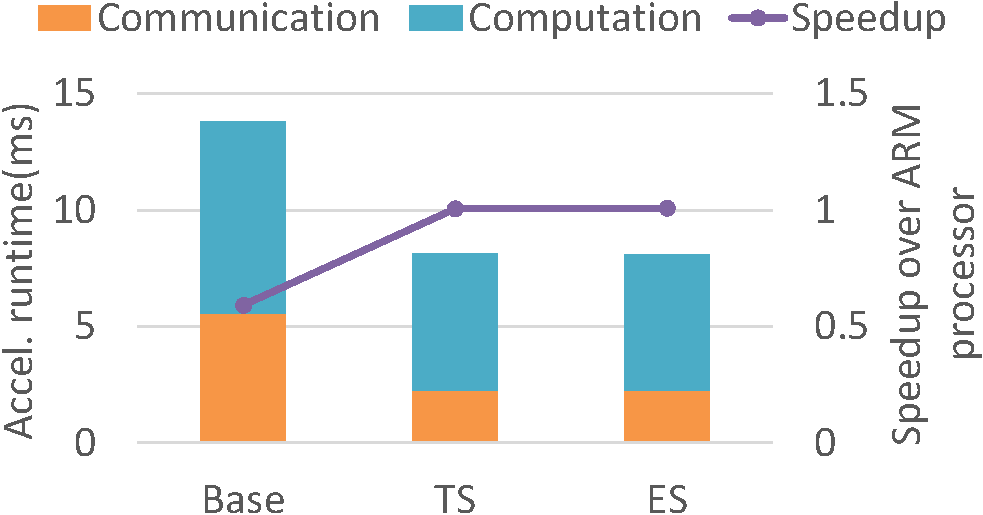
\includegraphics[width=0.45\textwidth]{mm-cp}
	}
	\subfigure[FIR]{%
		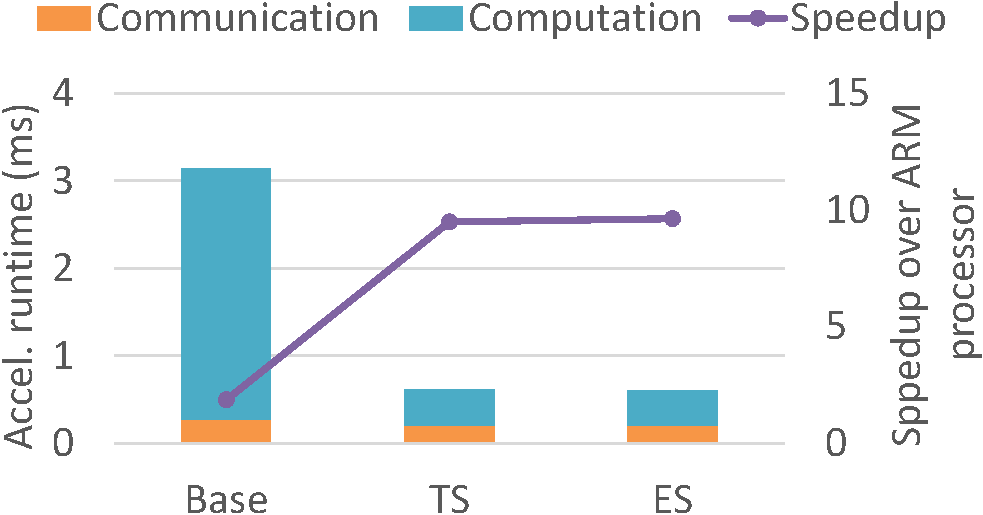
\includegraphics[width=0.45\textwidth]{fir-cp}
	}
    \hfill
	\subfigure[SE]{%
		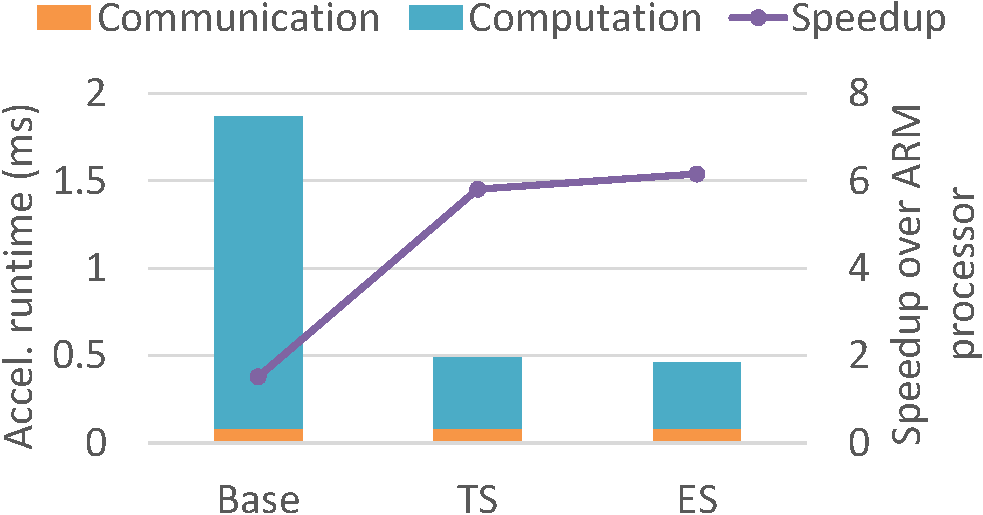
\includegraphics[width=0.45\textwidth]{se-cp}
	}
	\subfigure[KM]{%
		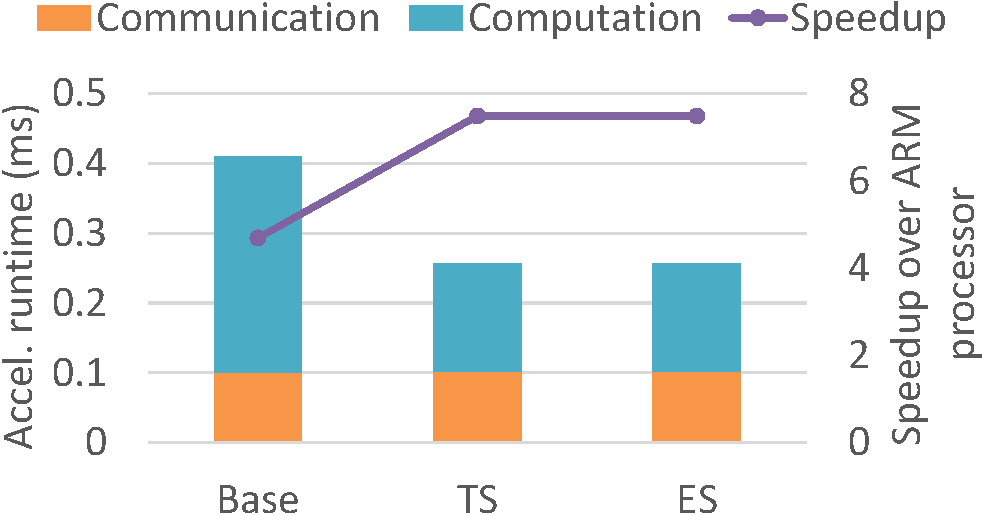
\includegraphics[width=0.45\textwidth]{km-cp}
	}
    \caption{Customized FPGA Loop Accelerator Performance Comparison}
	\label{fig:DSE}
\end{figure}

Finally, the FPGA resource consumption of the resulting accelerators are also compared. As block RAM is the resource bottleneck of the SCGRA overlay based FPGA accelerator design as mentioned in experiments in \chapref{chapter:overlay}, only block RAM resource consumption is presented in \figref{fig:BRAM-cp} to save the space. As shown in the figure, accelerators with random configurations may consume larger resource with worse performance. Compared to the accelerators produced using ES, the accelerators generated using TS typically consume less block RAM resource while achieving similar performance.

\begin{figure}[htb]
    \centering
    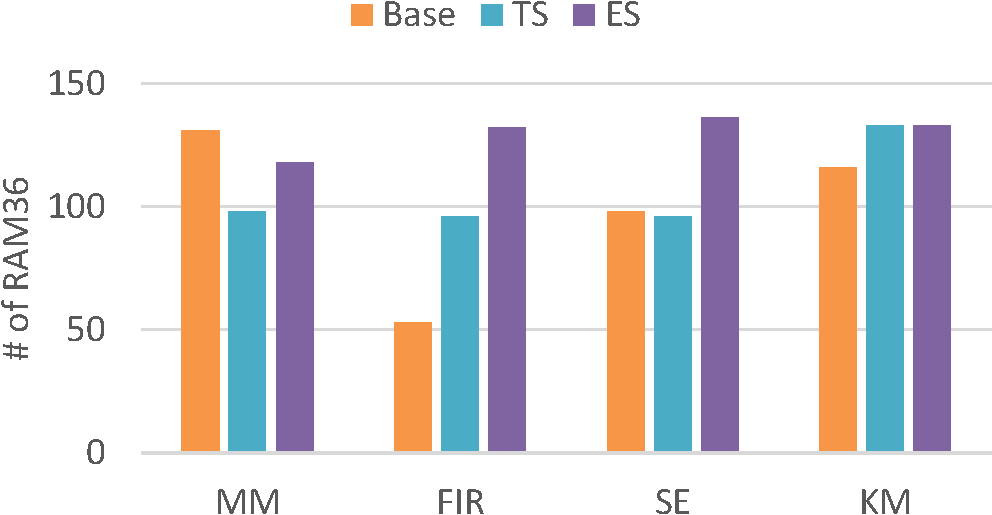
\includegraphics[width=0.65\textwidth]{BRAM-cp}
    \caption{Block RAM Consumption Comparison}
    \label{fig:BRAM-cp}
\end{figure}

\section{Summary}
In this work, an automatic nested loop accelerator customization framework that is based on a soft coarse-grained reconfigurable array overlay is presented. By taking advantage of the regularity of the SCGRA overlay, a two-step customization method is proposed for intensive system customization specific to the given user application. According to the experiments, it can be performed efficiently, resulting in up to \num{5} times performance improvement over solutions without customization at the cost of \num{10} to \num{20} minutes additional tools run time (The run time here means the customization time. If the configuration of the customized accelerator doesn't exist in the library, additional implementation time is required). Overall, the framework is able to generate accelerators that achieve up to \num{10} times speed up over software running on the host processor, resulting in a high design productivity experience for software programmers.
